\newpage
\section{Implementation} 
The hardware description of the implemented game pong is divided into six modules. Firstly the video controller, which implements the VGA respectively HDMI interface, provides the functionality to display the video output on a monitor. Two modules generate the inputs for the movement of the paddles. The right paddle is controlled by the debounced up and down buttons of the board and the right paddle is controlled by the computer opponent. Additionally the image generator creates all required objects like the ball and paddles as well as their movement. Furthermore the match controller manages the interactions between the objects and the state of the match itself. Lastly the audio output is created by the sound generator module.
	\subsection{Video Controller}
    The video controller provides an interface for the image generator so objects can easily be displayed on a monitor. Thereby it makes the coordinates of the current pixel available and hides all additional requirements of the protocol like timing. The point of origin of the pixel matrix is located at the top left corner of the monitor. Because our group has access to the Atlys Spartan-6 board with HDMI connector as well as the Nexys 4 board with VGA connector, we decided to implement a video controller for both protocols, so the remaining modules could be implemented using both boards. The main focus was laid on the above mentioned uniform interface for the image generator so the remaining development is independent of the used video controller.
        \subsubsection{VGA Controller}
        \subsubsection{HDMI Controller}
        	%%\section{HDMI}
%\subsection{Implementation}
For the first prototypes of the project VGA was used to stream the images to a screen. That needed to be changed because of two reasons: Firstly digital visual interfaces can get provide better resolution than analogue ones and secondly, and that is the actual main reason, the atlys board does not have a VGA port.

\subsubsection{HDMI - Principle of Operation}
HDMI(High Definition Multimedia Interface) is a digital interface which transport visual as well as audio data differential. The used encoding is the same as DVI called Transition-minimized differential signaling. TMDS is a kind of 8b/10b encoding but not the actual 8b/10b used by PCIE. It is optimized to create as less as possible transitions. Fast transitions are the main cause for electromagnetic interference which couples the twisted pair connection. \newline
The TMDS encoder transforms the actual bits with the previous bits with a XOR or a XNOR function. It takes always the one which causes less transitions. This transformation happens for the 8 data bits while the ninth bit encodes which operation was used. Additionally the sustained average DC level should stay similar. Therefore the encoder can invert the data to even out the balance of ones and zeros. This is saved in the tenth bit. \newline
Because of the fact that a HDMI connector just have 19 Pins, the data is transferred sequentially at a higher clockspeed. The first 12 Pins are for the data and the clock. For each color(RGB) and the clock there is a differential pair with one shield connection. That means that the bits have to be transferred with a 10 times faster clock than the clock which generates the pixel.



\subsubsection{HDMI with Spartan6 FPGAs on Atlys Boards}
The Atlys Board which is used in the project got 4 HDMI ports. The one which is called J2 is a usual Type A HDMI Connector. With this information it is possible to get the right constraints out of the following table(\ref{hdmi_constraints}).

\begin{figure}[h!]
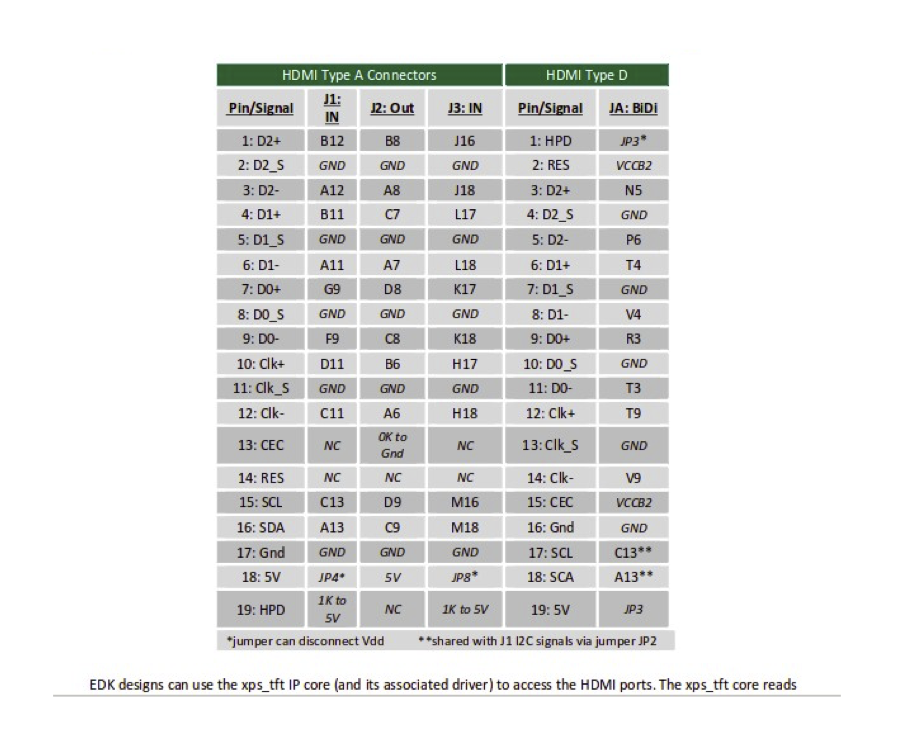
\includegraphics[scale=1.1]{images/hdmi_constraints.png} 

\caption{Constraints for HDMI(out of the Atlys User Manual)}
\label{hdmi_constraints}
\end{figure}

The actual design for the HDMI interface is shown in \ref{hdmi_design}. 
\begin{figure}[h!]
	\centering
	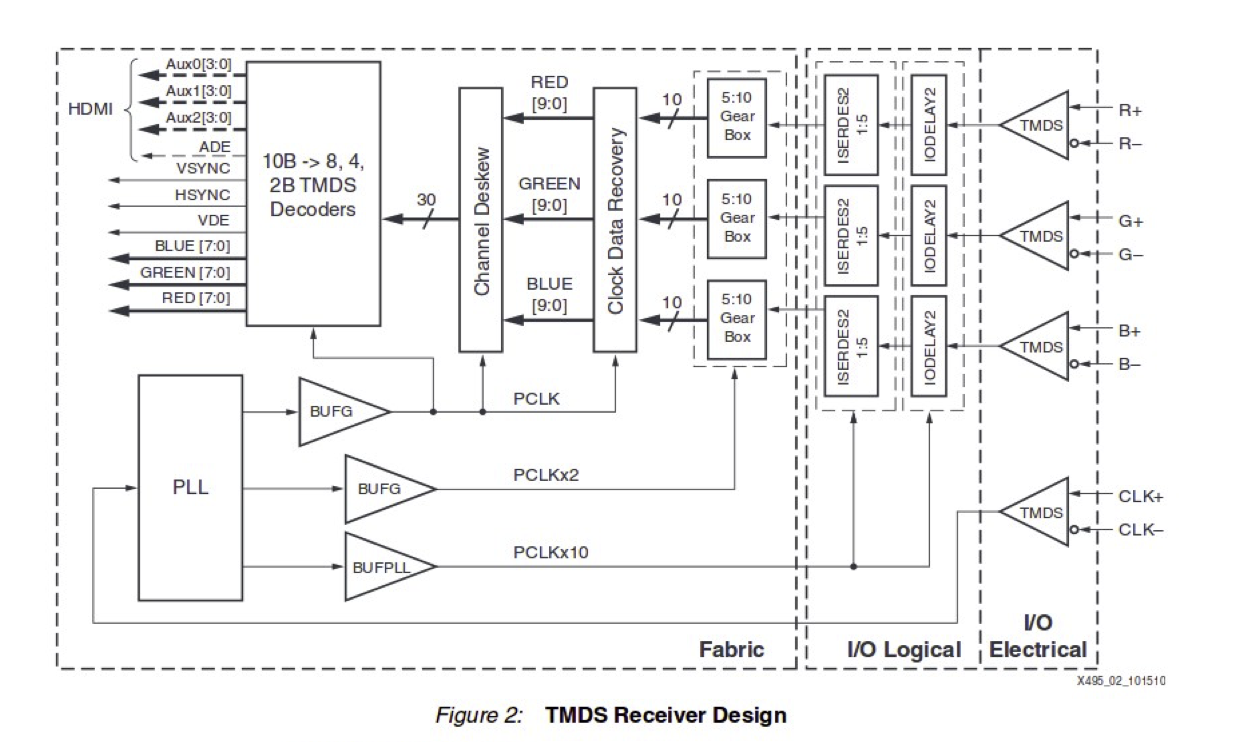
\includegraphics[scale=0.7]{images/hdmi_design.png}

\caption{Design how to build a HDMI interface(out of the TMDS User Interface Manual for Spartan6)}
\label{hdmi_design}
\end{figure}
This is a reference design by Xilinx itself. In the presented design the audio HDMI interface was not used, so ignore this part. Because of that there are just the video signals and the pixel clock there to mention. At first the RGB data is encoded by the TMDS module like it was described in the sections before. For a well synchronized transfer we need at the same time a perfectly timed pixel clock at a speed of 74.25 MHz. Because 74.25 MHz is hard to reach out of 100 MHz, 75 MHz were taken and it still worked fine. This clock was needed to be created by the clockwizard IP. In the next parts the TMDS encoded RGB data is converted and serialized into the differential TMDS signals. Because of the serialization we need a 10 times faster clock which is created out of the PLL shown in the schematic. Additionally to RGB data the clock is sent as well for synchronization.


        	%\section{HDMI}
%\subsection{Implementation}
For the first prototypes of the project VGA was used to stream the images to a screen. That needed to be changed because of two reasons: Firstly digital visual interfaces can get provide better resolution than analogue ones and secondly, and that is the actual main reason, the atlys board does not have a VGA port.

\subsubsection{HDMI - Principle of Operation}
HDMI(High Definition Multimedia Interface) is a digital interface which transport visual as well as audio data differential. The used encoding is the same as DVI called Transition-minimized differential signaling. TMDS is a kind of 8b/10b encoding but not the actual 8b/10b used by PCIE. It is optimized to create as less as possible transitions. Fast transitions are the main cause for electromagnetic interference which couples the twisted pair connection. \newline
The TMDS encoder transforms the actual bits with the previous bits with a XOR or a XNOR function. It takes always the one which causes less transitions. This transformation happens for the 8 data bits while the ninth bit encodes which operation was used. Additionally the sustained average DC level should stay similar. Therefore the encoder can invert the data to even out the balance of ones and zeros. This is saved in the tenth bit. \newline
Because of the fact that a HDMI connector just have 19 Pins, the data is transferred sequentially at a higher clockspeed. The first 12 Pins are for the data and the clock. For each color(RGB) and the clock there is a differential pair with one shield connection. That means that the bits have to be transferred with a 10 times faster clock than the clock which generates the pixel.



\subsubsection{HDMI with Spartan6 FPGAs on Atlys Boards}
The Atlys Board which is used in the project got 4 HDMI ports. The one which is called J2 is a usual Type A HDMI Connector. With this information it is possible to get the right constraints out of the following table(\ref{hdmi_constraints}).

\begin{figure}[h]
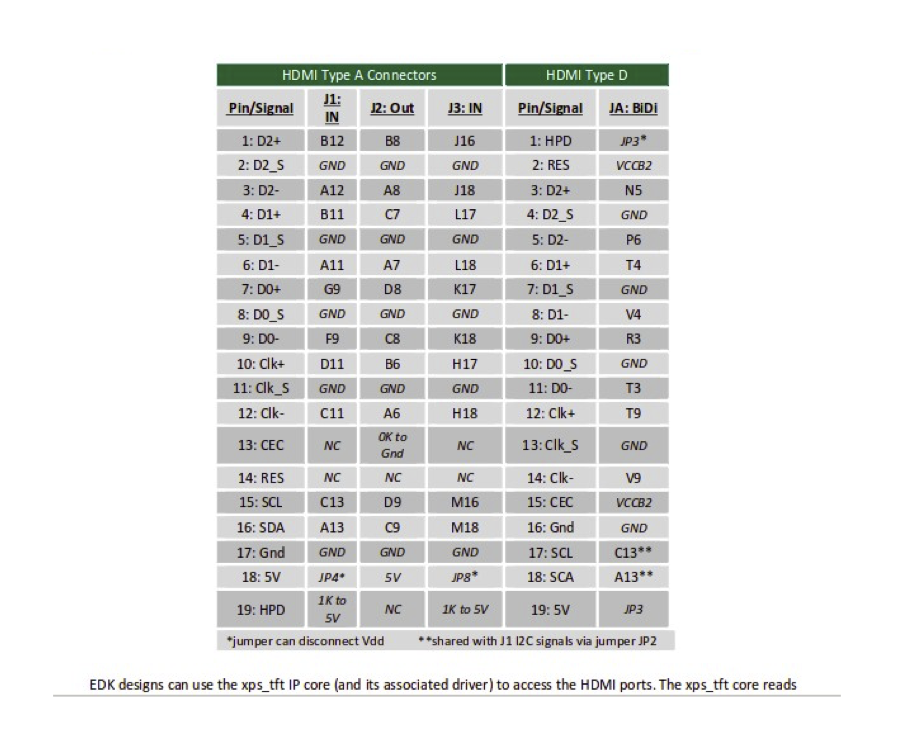
\includegraphics[scale=1.1]{images/hdmi_constraints.png} 

\caption{Constraints for HDMI(out of the Atlys User Manual)}
\label{hdmi_constraints}
\end{figure}

The actual design for the HDMI interface is shown in \ref{hdmi_design}. 
\begin{figure}[h]
	\centering
	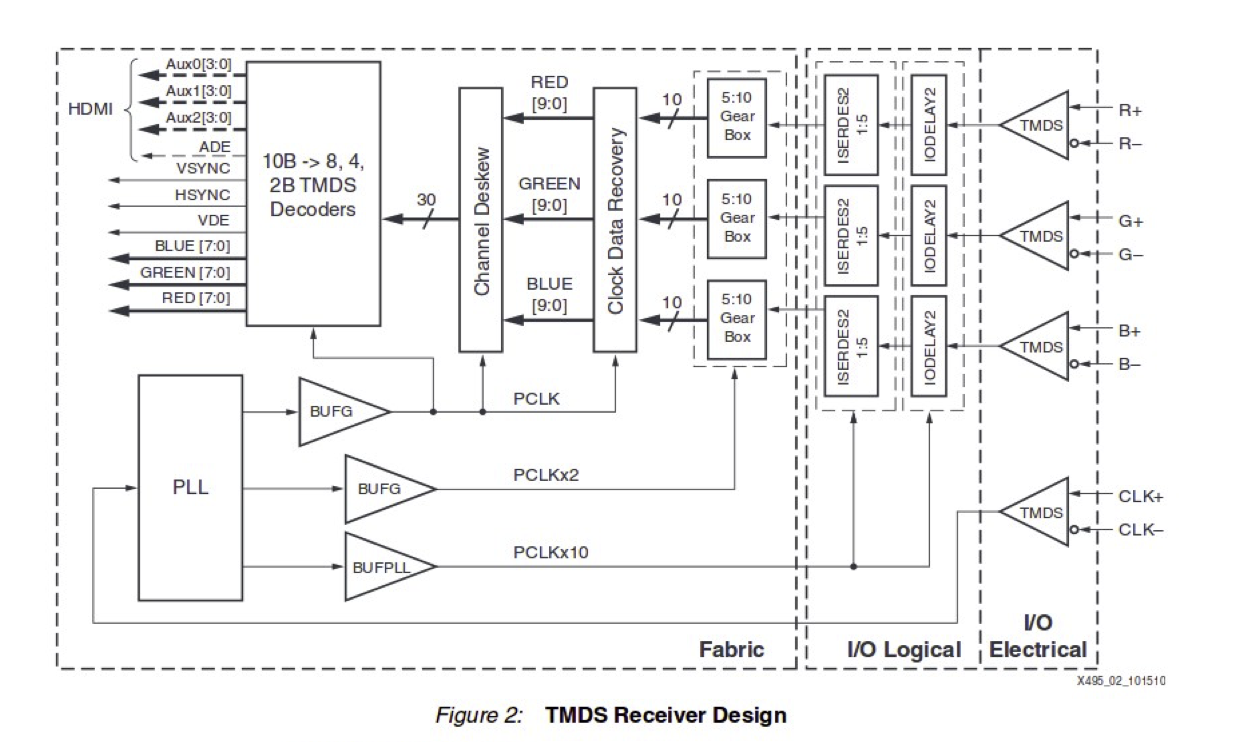
\includegraphics[scale=0.7]{images/hdmi_design.png}

\caption{Design how to build a HDMI interface(out of the TMDS User Interface Manual for Spartan6)}
\label{hdmi_design}
\end{figure}
This is a reference design by Xilinx itself. In the presented design the audio HDMI interface was not used, so ignore this part. Because of that there are just the video signals and the pixel clock there to mention. At first the RGB data is encoded by the TMDS module like it was described in the sections before. For a well synchronized transfer we need at the same time a perfectly timed pixel clock at a speed of 74.25 MHz. Because 74.25 MHz is hard to reach out of 100 MHz, 75 MHz were taken and it still worked fine. This clock was needed to be created by the clockwizard IP. In the next parts the TMDS encoded RGB data is converted and serialized into the differential TMDS signals. Because of the serialization we need a 10 times faster clock which is created out of the PLL shown in the schematic. Additionally to RGB data the clock is sent as well for synchronization.


    \subsection{Debouncer}
    \subsection{Computer Opponent}
    \subsection{Image Generator}
    
  %this figure was redundant, therefore it has been removed
%	\begin{figure}[here]
%		\centering
%		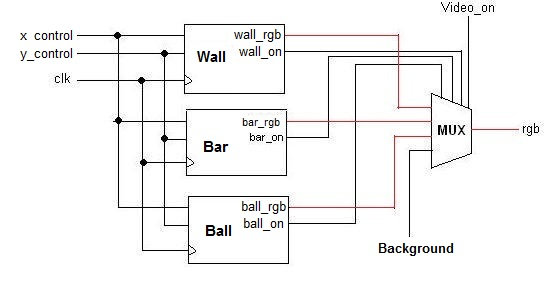
\includegraphics[scale=0.7]{images/img_gen.jpg}
%		\caption{Schematic of the Image Generator}
%		\label{img_gen}
%	\end{figure}
        The Image Generator takes inputs from the players and outputs the video that can be displayed through the HDMI interface of the Atlys board. The panels shown in figure \ref{ball_wall_panel} are submodules of the module \texttt{image\_generator\_c}.
		This module calculates the movement of the ball and movement the two panels that are controlled by the players. 
		
		The movement of the ball is done by the \texttt{ball\_c} module.
		After a well determined time frame, the ball's movement direction is determined and the next \texttt{x\_pos} and \texttt{y\_pos} are either incremented or decremented. 
		
		The module \texttt{panel\_c} determines the y-coordinate of on panel based on the player input. For instance, pressing \texttt{btn\_up} increments the \texttt{y\_pos} signal if the panel did not reach the top edge already. 


    \subsection{Match Controller}
    
    \newpage
	  \subsection{Sound Generator}
				In order to generate sound, we used the on board LM4550 chip. Figure \ref{snd_gen} shows the block diagram of the sound generator. This module takes in the sound events from the Match Controller module (i.e when sound generation should take place), reads a sound effect from a ROM and sends it to the LM4550 chip that in turn outputs the sound effect to a connected speaker.
				
				The inputs to the \texttt{snd\_gen\_c} include a \texttt{clk}, an active low reset, a serial data in line \texttt{sdata\_in}, a 12.288 MHz bit clock from the AC97 chip, 3 bit \texttt{snd\_eff} signal and 5 bit \texttt{volume} control (will be connected to the switches of the Atlys board).
				
				The module's output include a \texttt{sync} signal, serial data output \texttt{sdata\_out} and an AC97 active low reset that initializes the AC97 (LM4550) chip. 
				
				Internally, the \texttt{snd\_gen\_c} module contains an AC97 controller and an AC97CMD submodules.
				\begin{itemize}
				\item \textbf{AC97 controller:} implements the AC Link serial interface protocol. Figure \ref{LM4550_protocol} shows an AC bidirectional audio frame, whereas figure \ref{LM4550_output_frame} shows an AC output audio frame. In this project, we will be using the LM4550 chip for output only, however, the input audio frame (not shown here) has also been implemented for testing reasons. The next paragraph is a brief description of the AC link interface protocol. For more details about the AC97 link serial interface protocol, see \url{http://www.ti.com/lit/ds/symlink/lm4550.pdf}
				
				The AC Link Output Frame carries control and PCM data to the LM4550 control registers and stereo DAC. Output Frames are carried on the \texttt{sdata\_out} signal which is an output from the AC97 Controller and an input to the LM4550 codec. As shown in Figure \ref{LM4550_output_frame}, Output Frames are constructed from thirteen time slots: one Tag Slot followed by twelve Data Slots. Each Frame consists of 256 bits with each of the twelve Data Slots containing 20 bits. Input and Output Frames are aligned to the same SYNC transition.
					
			\begin{figure}[here!]
			\centering
				\begin{subfigure}{0.6\textwidth}
					\centering
					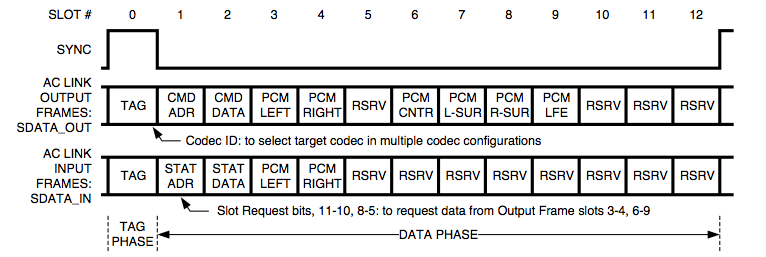
\includegraphics[scale=1]{images/LM4550_protocol.png}
					\caption{AC link bidirectional frame}
					\label{LM4550_protocol}
				\end{subfigure}
				\hfill
				\begin{subfigure}{0.6\textwidth}
					\centering
					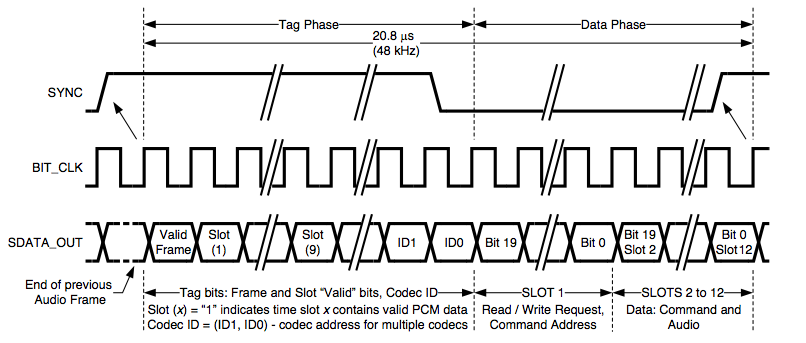
\includegraphics[scale=1]{images/LM4550_output_frame.png}
					\caption{AC link output audio frame}
					\label{LM4550_output_frame}
				\end{subfigure}
				\hfill
				\begin{subfigure}[b]{0.6\textwidth}
					\centering
					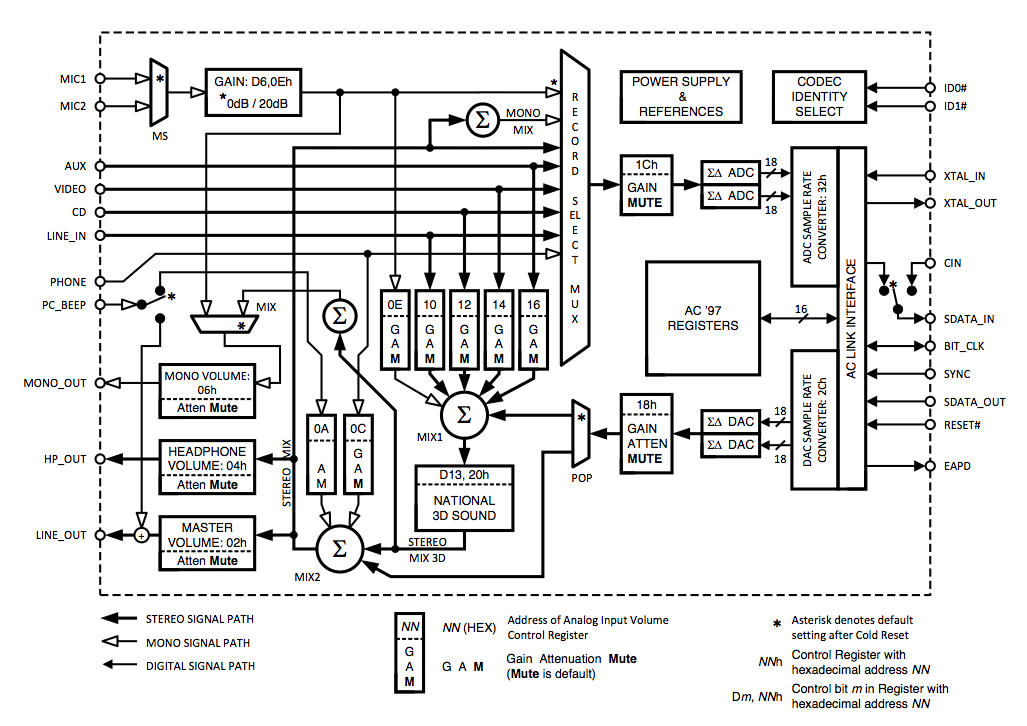
\includegraphics[scale=0.8]{images/LM4550_innen.png}
					\caption{Block diagram of LM4550 chip. Red line is the path from FPGA output to \texttt{HP\_OUT}. All registers along this path need to be configured.}
					\label{LM4550_innen}
				\end{subfigure}
				
			\caption{AC link serial interface protocol} 
			\end{figure}
				\item \textbf{AC97CMD command state machine:} is a state machine that creates the control data based on the inputs \texttt{snd\_eff} and \texttt{volume} and passes it to the AC97 Controller. This control data controls among others the volume of the output audio and the DAC sample rate. Figure \ref{LM4550_innen} shows the path of the audio data that gets transferred within the LM4550 chip and the registers that need to be configured along this path. The following code was extracted from the file \texttt{a97cmd\_fsm.vhd} that implements the state machine necessary to configure the registers of the LM4550 chip. It shows an example of how to activate the output \texttt{HP\_OUT}. As shown in figure \ref{LM4550_innen} \texttt{LINE\_OUT} is muted by default. 
				
%				\begin{figure}[h]
%					\centering
%					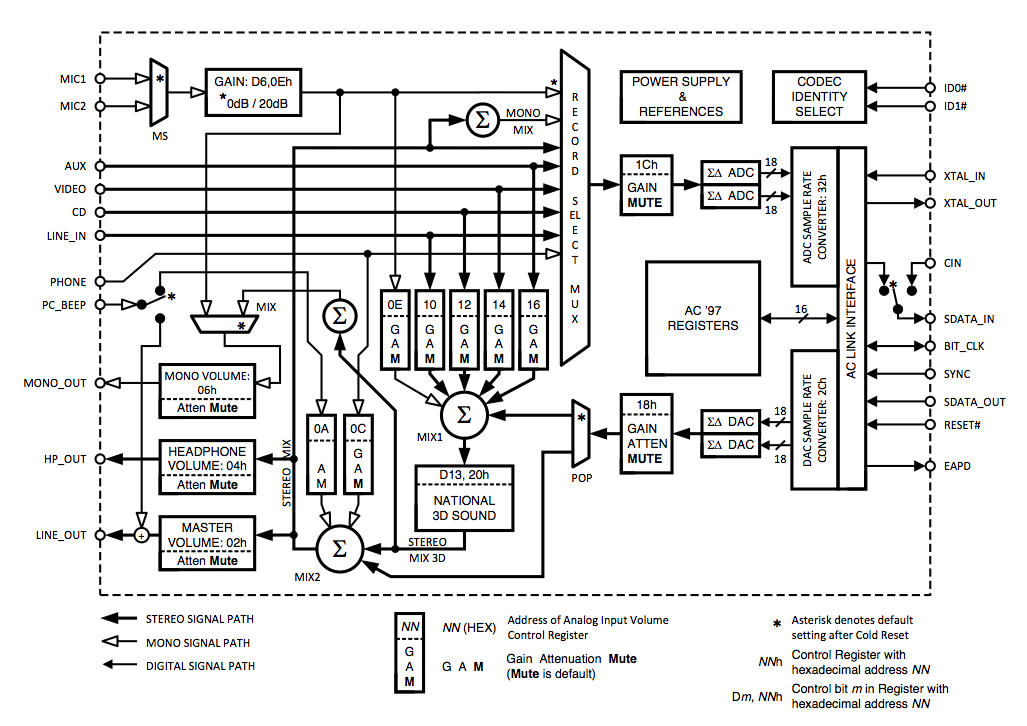
\includegraphics[scale=1]{images/LM4550_innen.png}
%					\caption{Block diagram of LM4550 chip. Red line is the path from FPGA output to \texttt{HP\_OUT}. All registers along this path need to be configured.}
%					\label{LM4550_innen}
%				\end{figure}
$\cdots$
\begin{lstlisting}
process (next_state, cur_state, atten)
    begin
        case cur_state is
    	    when S0 =>
            cmd <= X"02_8000";  -- master volume    0 0000->0dB atten, 
                                               1 1111->46.5dB atten						
                next\_state <= S2;
            when S1 => 
                                               -- HP_OUT volume
                cmd <= X"04" & "000" & atten & "000" & atten;	
                next\_state <= S4;
            when S2 => 			
		
\end{lstlisting}
$\cdots$\\
The AC97CMD module also reads the audio sound effects from a ROM that gets initialized when the FPGA is programmed. The right sound effect is chosen according to the signal \texttt{snd\_eff}.
				\end{itemize}
		  
